\chapter{Mesure du comportement de la maquette avec la régulation de position MIMO}

\section{Introduction}
À la suite des différentes modifications apportées à la régulation de position, une mesure du comportement général de la maquette a été réalisée. Elle est présentée dans ce chapitre.

\section{Mesure du système}
Comparées aux mesures précédentes, celles présentées ici portent sur les grandeurs modales. Elles se concentrent donc sur le pompage, le tangage et le roulis. Une mesure du comportement par inducteur a également été réalisée.

Deux mesures ont été effectuées :

\begin{itemize}
    \item une première mesure sans intervention extérieure.
    \item une seconde mesure avec l'ajout d'une perturbation.
\end{itemize}

La perturbation consiste simplement à appuyer sur l'un des côtés de la maquette.

La mesure est réalisée comme dans l'\autoref{annexe:MesureComplete}, mais en y ajoutant les composantes de la régulation MIMO :

\begin{minted}{c}
    UartCounter++;
    if (UartCounter >= 250)
    {
        UartCounter = 0;

        if(!TelemetryReady)
        {
            TelemetrySnap[0]  = frameCnt;
            TelemetrySnap[1]  = (float)state;

            TelemetrySnap[2]  = qm_ref[0] * 1000.0f;
            TelemetrySnap[3]  = qm_ref[1] * 1000.0f;
            TelemetrySnap[4]  = qm_ref[2] * 1000.0f;

            TelemetrySnap[5]  = qm[0] * 1000.0f;
            TelemetrySnap[6]  = qm[1] * 1000.0f;
            TelemetrySnap[7]  = qm[2] * 1000.0f;

            TelemetrySnap[8]  = vm_est[0] * 1000.0f;
            TelemetrySnap[9]  = vm_est[1] * 1000.0f;
            TelemetrySnap[10] = vm_est[2] * 1000.0f;

            TelemetrySnap[11] = u_cmd[0];
            TelemetrySnap[12] = u_cmd[1];
            TelemetrySnap[13] = u_cmd[2];

            TelemetrySnap[14] = u_sat[0];
            TelemetrySnap[15] = u_sat[1];
            TelemetrySnap[16] = u_sat[2];

            TelemetrySnap[17] = LQI_EPS[0] * eps_m[0];
            TelemetrySnap[18] = LQI_EPS[1] * eps_m[1];
            TelemetrySnap[19] = LQI_EPS[2] * eps_m[2];

            TelemetrySnap[20] = Position1 * 1000.0f;
            TelemetrySnap[21] = Position2 * 1000.0f;
            TelemetrySnap[22] = Position3 * 1000.0f;
            TelemetrySnap[23] = Position4 * 1000.0f;

            TelemetrySnap[24] = fc1;
            TelemetrySnap[25] = fc2;
            TelemetrySnap[26] = fc3;
            TelemetrySnap[27] = fc4;

            TelemetrySnap[28] = Current1;
            TelemetrySnap[29] = Current2;
            TelemetrySnap[30] = Current3;
            TelemetrySnap[31] = Current4;

            TelemetryReady = true;
        }

        frameCnt += 1.0f;
    }
\end{minted}

\subsection{Mesure sans intervention extérieure}
Le profil du système dans l'espace, sans intervention, donne les résultats de la \autoref{fig:PompageSansIntervention} à la \autoref{fig:RoulisSansIntervention} :

\begin{figure}[H]
    \centering
    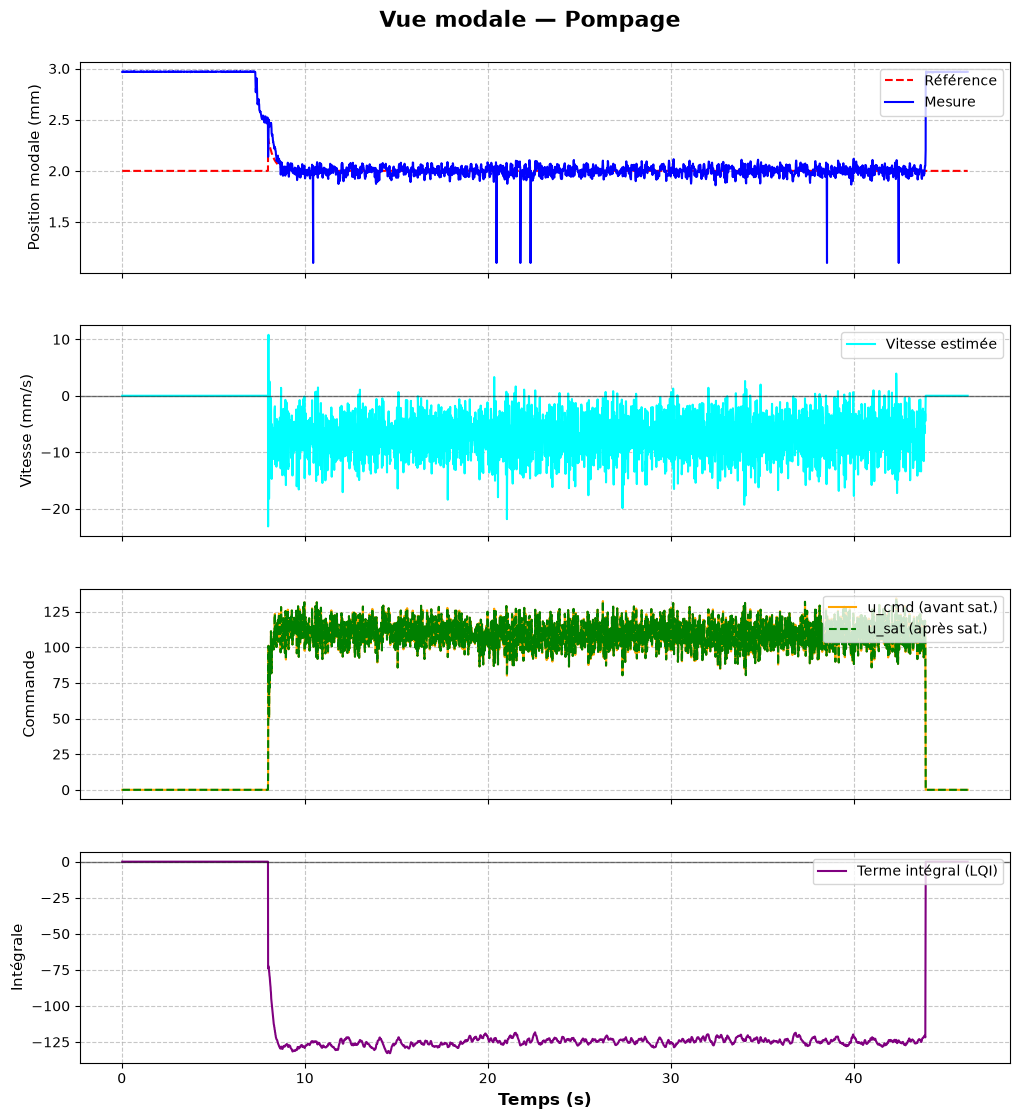
\includegraphics[width=1\linewidth]{assets/content/14-MesureMIMO/SansIntervention/Pompage.png}
    \caption{Comportement du pompage sans intervention extérieure}
    \label{fig:PompageSansIntervention}
\end{figure}

\begin{figure}[H]
    \centering
    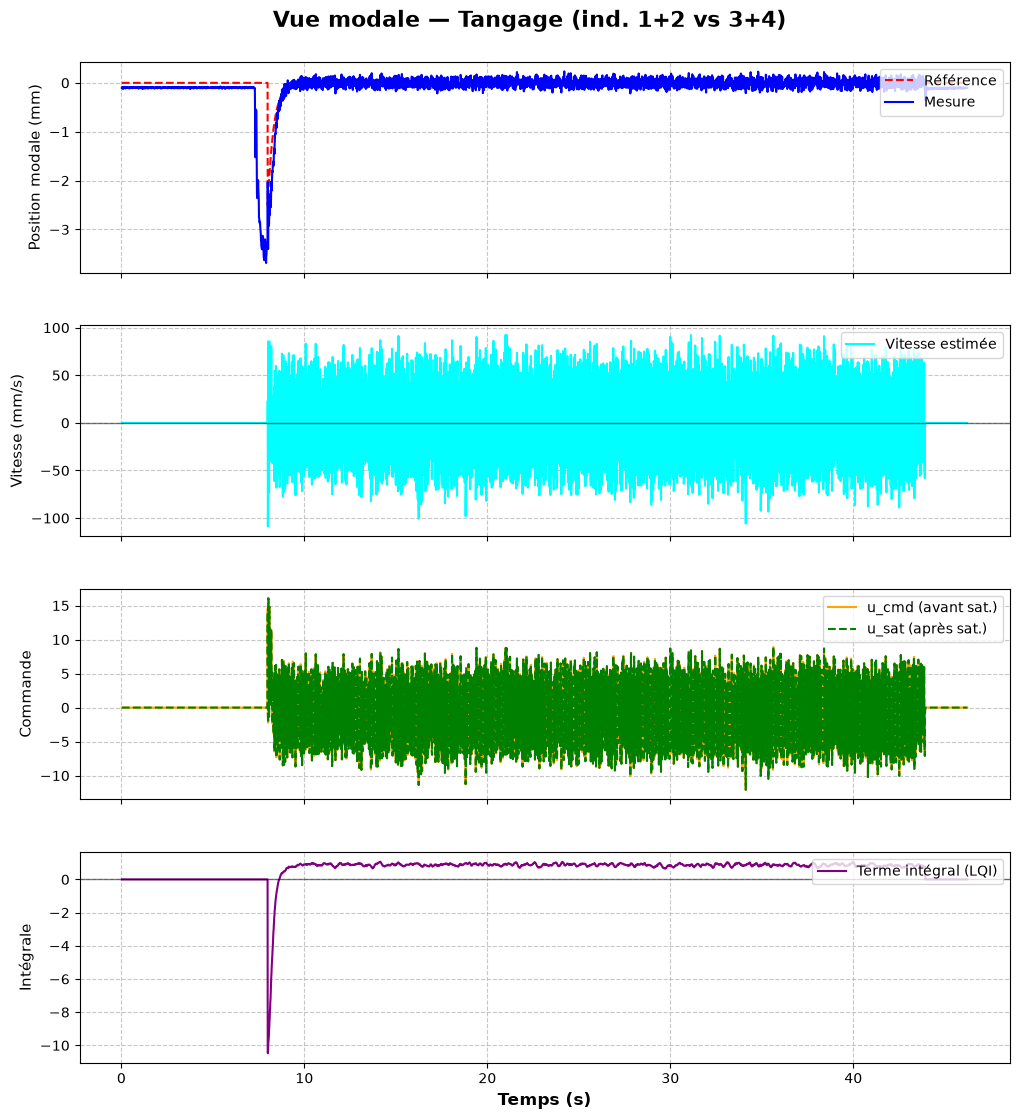
\includegraphics[width=1\linewidth]{assets/content/14-MesureMIMO/SansIntervention/Tangage.png}
    \caption{Comportement du tangage sans intervention extérieure}
    \label{fig:TangageSansIntervention}
\end{figure}

\begin{figure}[H]
    \centering
    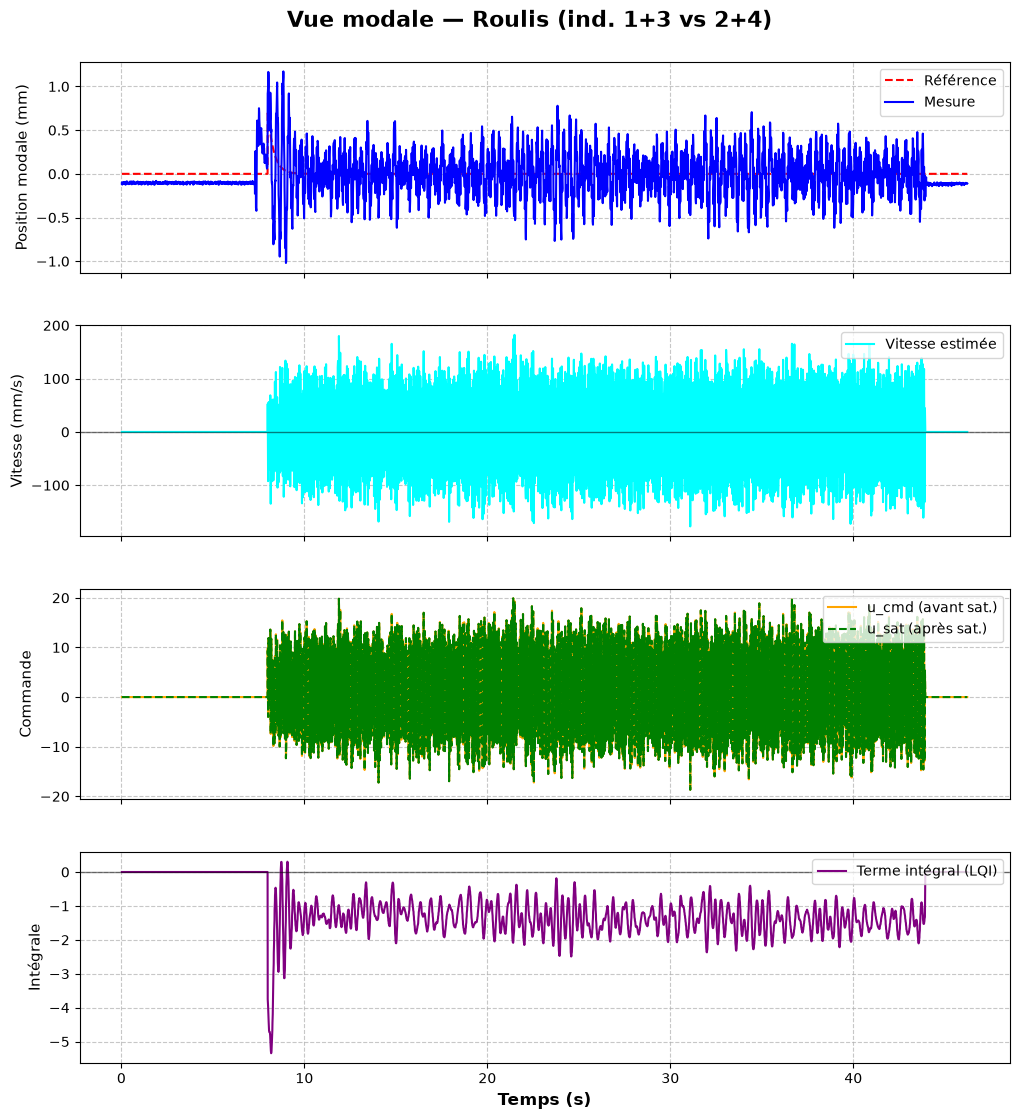
\includegraphics[width=1\linewidth]{assets/content/14-MesureMIMO/SansIntervention/Roulis.png}
    \caption{Comportement du roulis sans intervention extérieure}
    \label{fig:RoulisSansIntervention}
\end{figure}

Le comportement par inducteur, sans intervention, est présenté de la \autoref{fig:Ind1SansIntervention} à la \autoref{fig:Ind4SansIntervention} :

\begin{figure}[H]
    \centering
    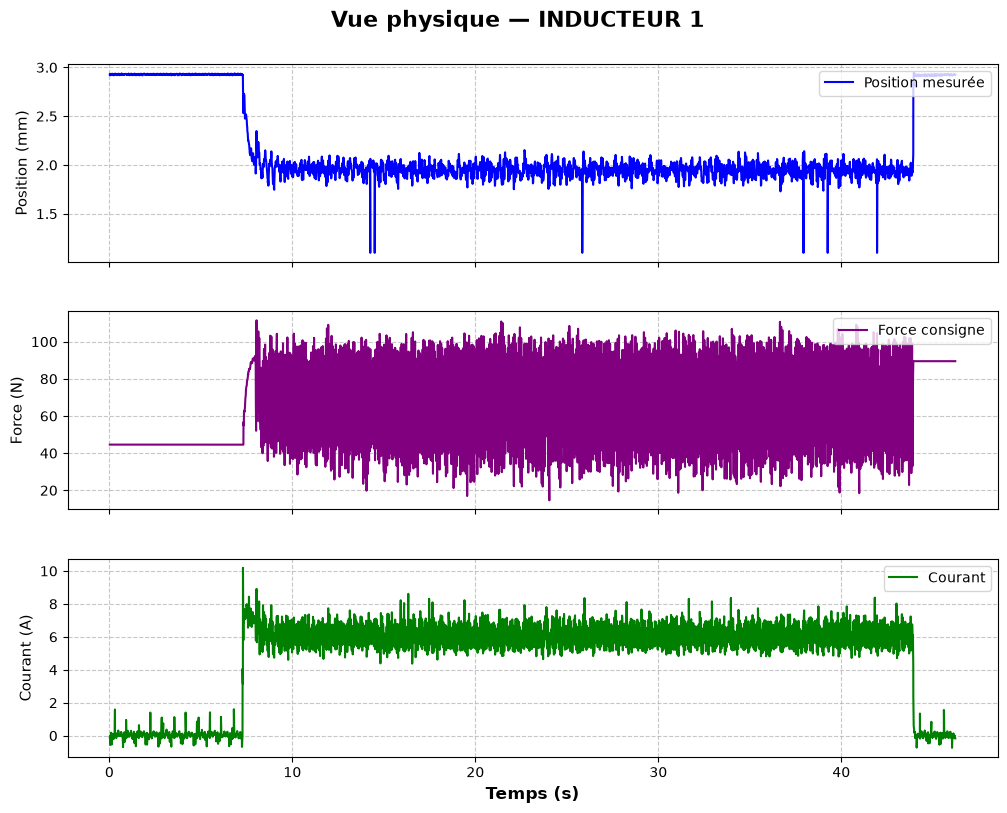
\includegraphics[width=1\linewidth]{assets/content/14-MesureMIMO/SansIntervention/Ind1.png}
    \caption{Comportement de l'inducteur 1 sans intervention extérieure}
    \label{fig:Ind1SansIntervention}
\end{figure}

\begin{figure}[H]
    \centering
    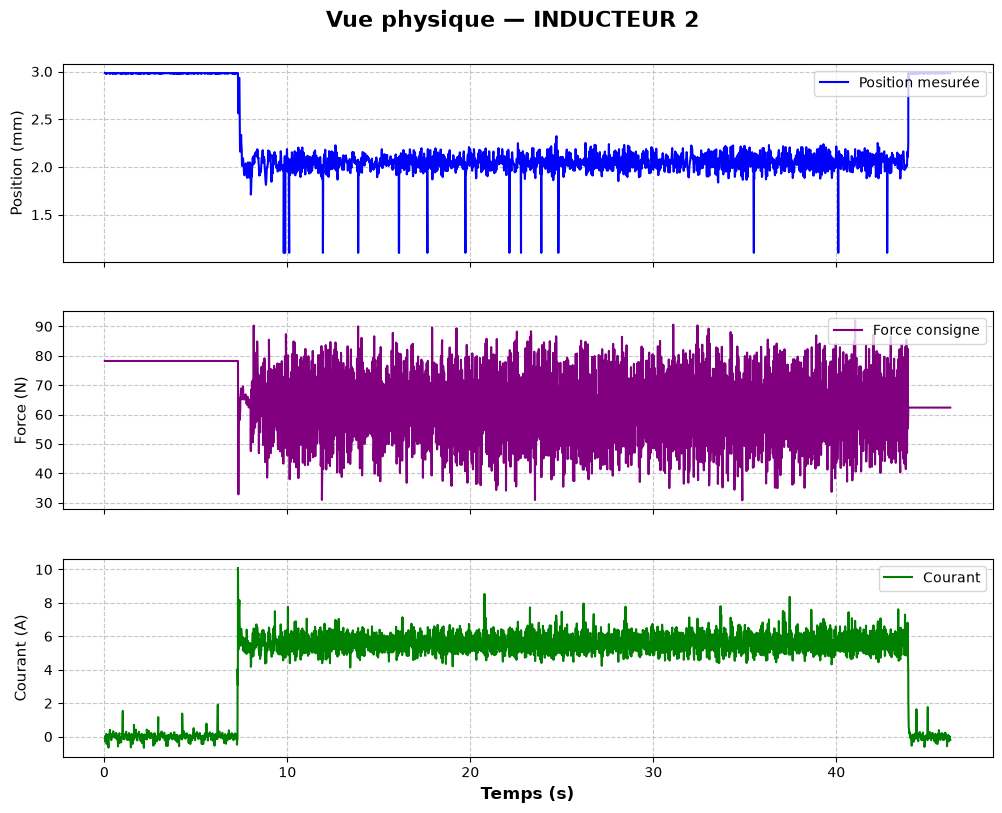
\includegraphics[width=1\linewidth]{assets/content/14-MesureMIMO/SansIntervention/Ind2.png}
    \caption{Comportement de l'inducteur 2 sans intervention extérieure}
    \label{fig:Ind2SansIntervention}
\end{figure}

\begin{figure}[H]
    \centering
    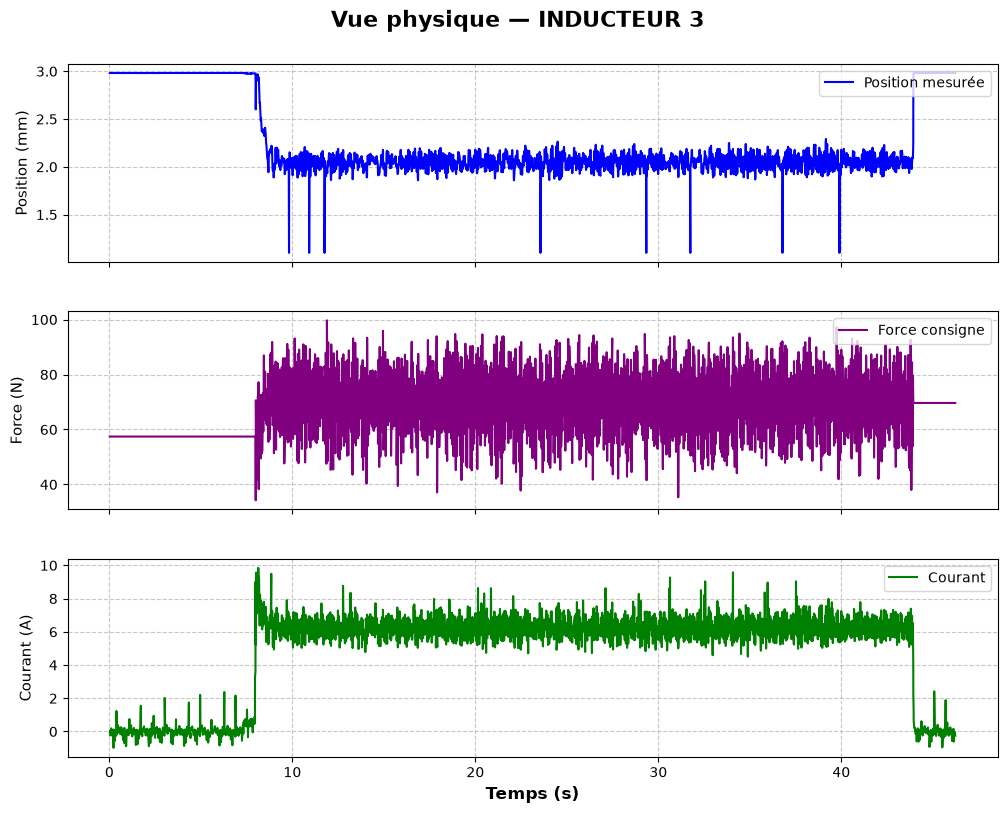
\includegraphics[width=1\linewidth]{assets/content/14-MesureMIMO/SansIntervention/Ind3.png}
    \caption{Comportement de l'inducteur 3 sans intervention extérieure}
    \label{fig:Ind3SansIntervention}
\end{figure}

\begin{figure}[H]
    \centering
    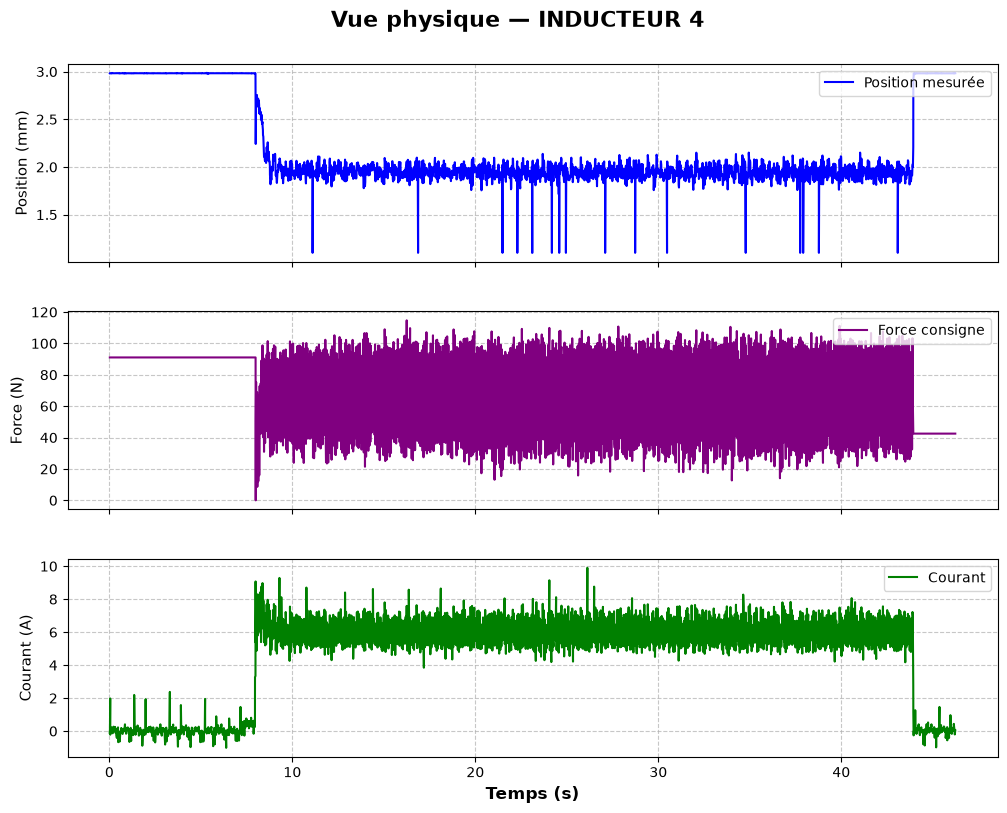
\includegraphics[width=1\linewidth]{assets/content/14-MesureMIMO/SansIntervention/Ind4.png}
    \caption{Comportement de l'inducteur 4 sans intervention extérieure}
    \label{fig:Ind4SansIntervention}
\end{figure}

Il est ensuite possible de se concentrer sur la force émise par chaque inducteur, présentée dans la \autoref{fig:ForceSansIntervention} :

\begin{figure}[H]
    \centering
    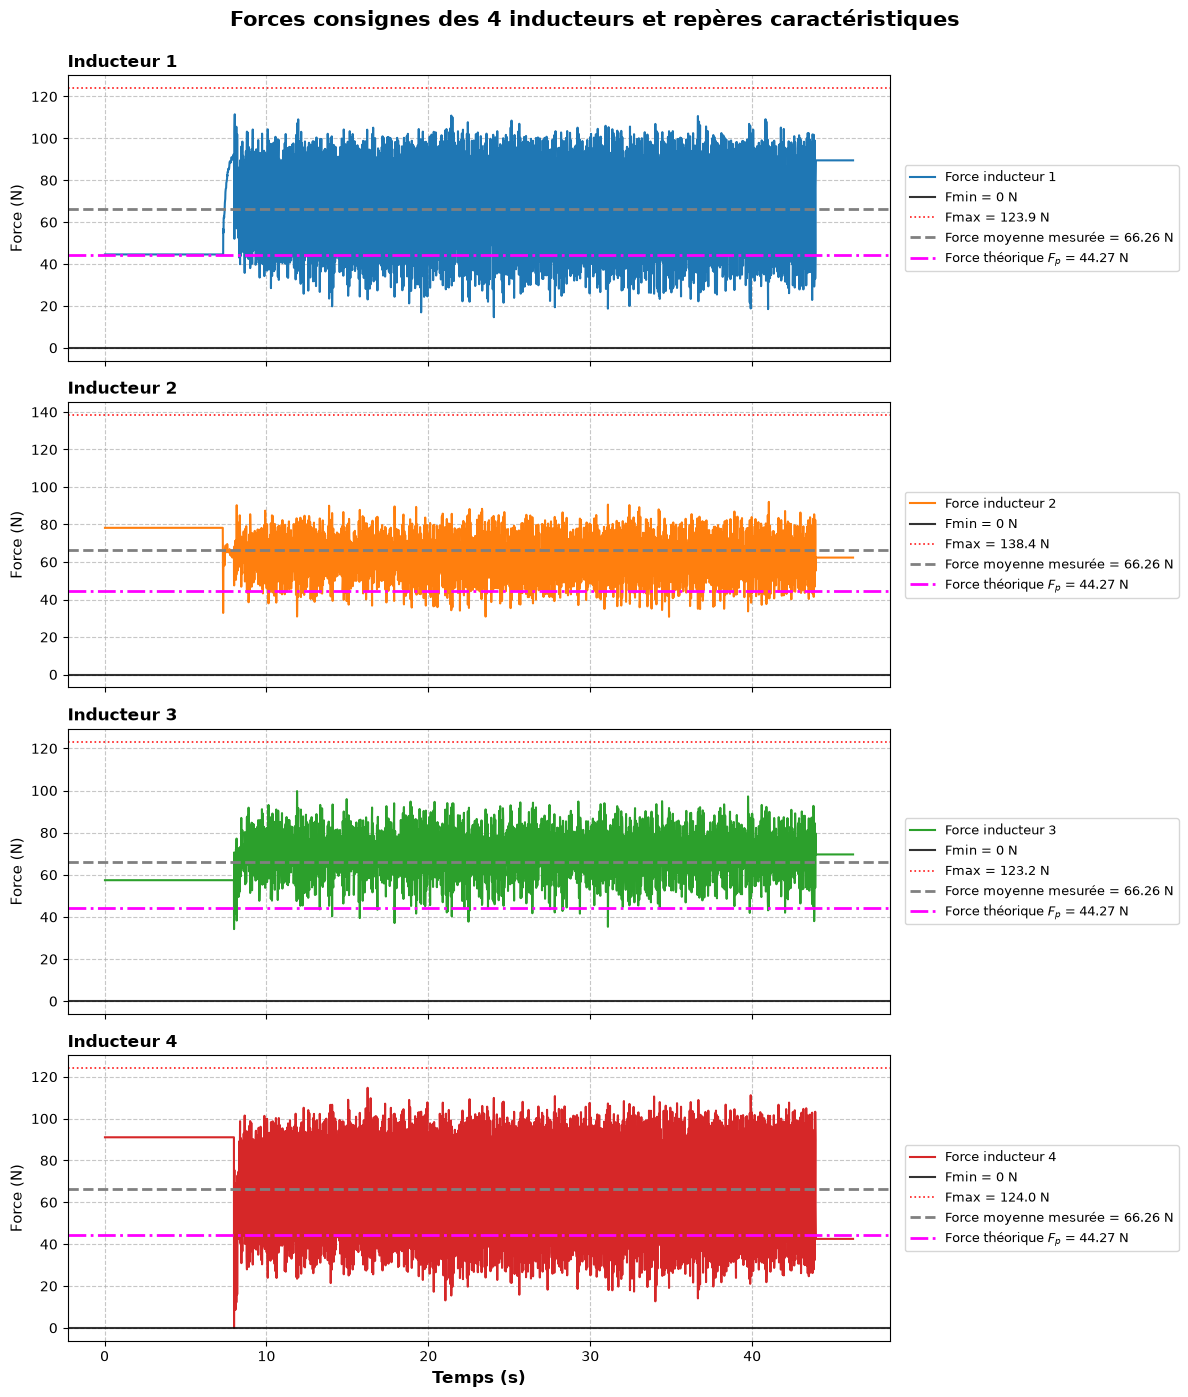
\includegraphics[width=1\linewidth]{assets/content/14-MesureMIMO/SansIntervention/Force.png}
    \caption{Comportement des forces sans intervention extérieure}
    \label{fig:ForceSansIntervention}
\end{figure}

L'écart entre la force théorique de pesanteur et la force réellement émise par le système peut alors être calculé, comme le montre le \autoref{tab:forces_inducteurs_v3} :

\begin{table}[htbp]
    \centering
    \begin{tabular}{l cccc}
        \toprule
        \textbf{Inducteur} & \makecell[c]{\textbf{Force moyenne}                         \\ \textbf{[N]}} & \makecell[c]{\textbf{Force théorique $F_p$} \\ \textbf{[N]}} & \makecell[c]{\textbf{Écart} \\ \textbf{[N]}} & \makecell[c]{\textbf{Écart} \\ \textbf{[\%]}} \\
        \midrule
        1                  & 64.44                               & 44.27 & 20.17 & 45.56 \\
        2                  & 64.90                               & 44.27 & 20.63 & 46.60 \\
        3                  & 67.25                               & 44.27 & 22.98 & 51.91 \\
        4                  & 68.46                               & 44.27 & 24.19 & 54.63 \\
        \bottomrule
    \end{tabular}
    \caption{Comparaison des forces moyennes et théoriques par inducteur, sans intervention}
    \label{tab:forces_inducteurs_v3}
\end{table}

\subsection{Mesure avec l'ajout d'une perturbation}
La seconde mesure montre comment le système réagit à l'ajout d'une perturbation.

Le profil du système dans l'espace, avec une perturbation, donne les résultats de la \autoref{fig:PompageOscillation} à la \autoref{fig:RoulisOscillation} :

\begin{figure}[H]
    \centering
    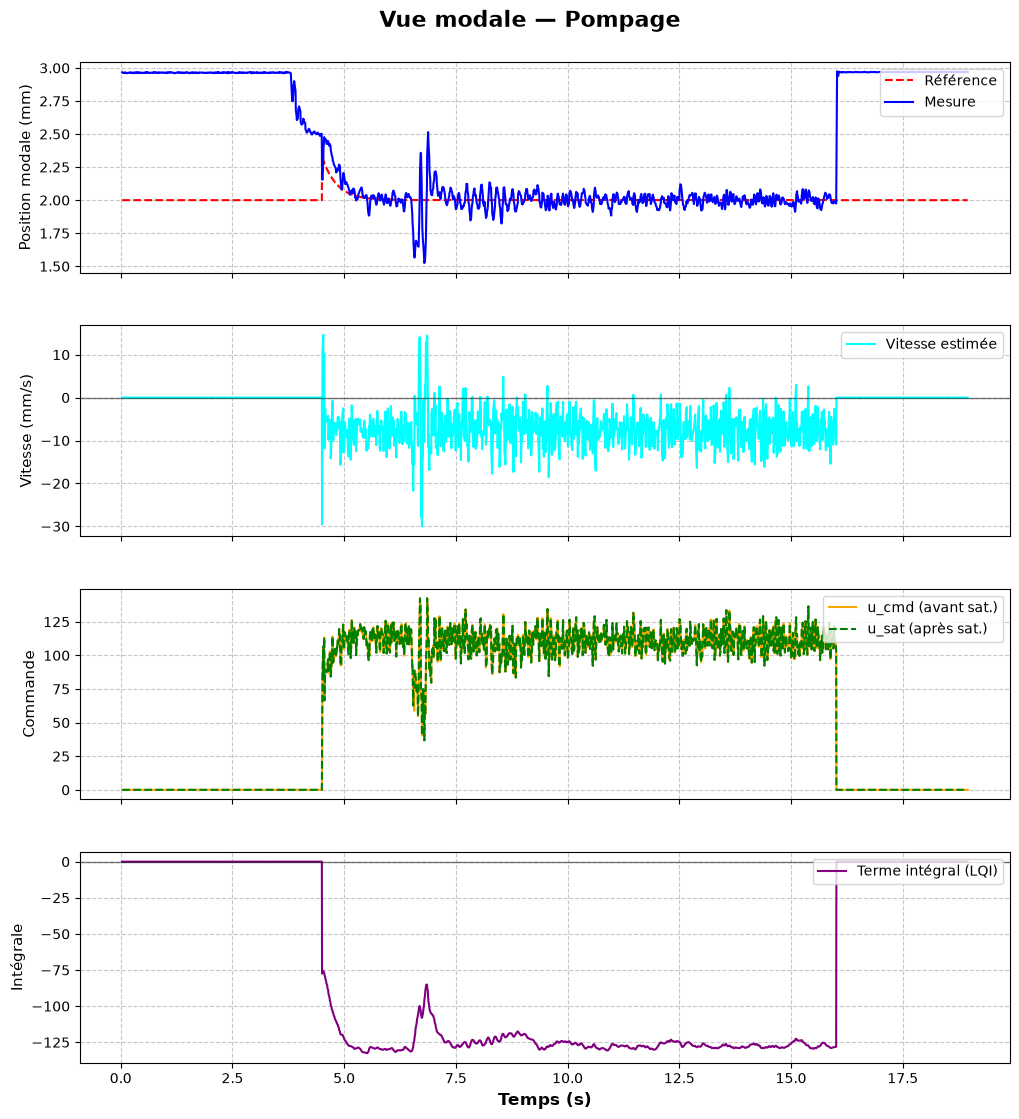
\includegraphics[width=1\linewidth]{assets/content/14-MesureMIMO/Oscillation/Pompage.png}
    \caption{Comportement du pompage avec une perturbation}
    \label{fig:PompageOscillation}
\end{figure}

\begin{figure}[H]
    \centering
    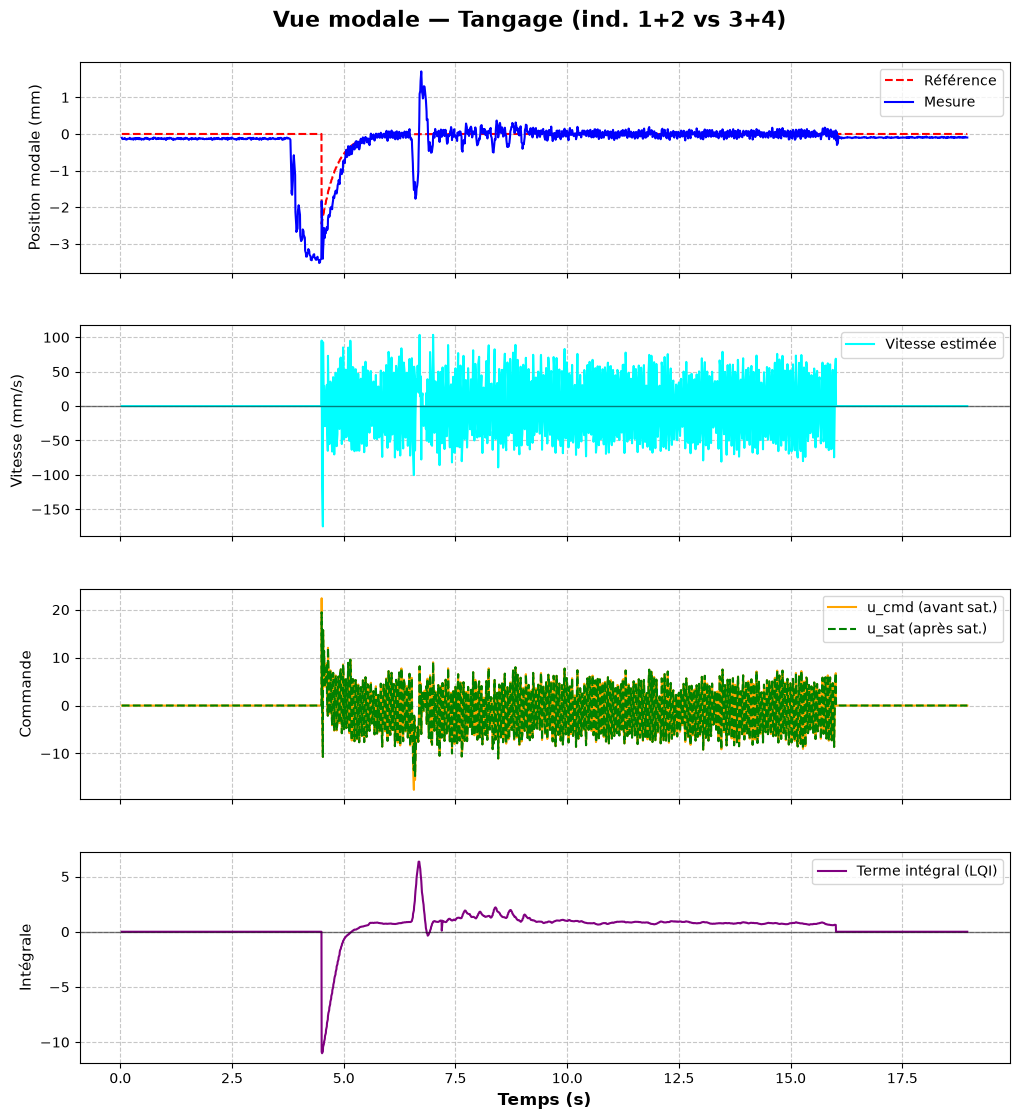
\includegraphics[width=1\linewidth]{assets/content/14-MesureMIMO/Oscillation/Tangage.png}
    \caption{Comportement du tangage avec une perturbation}
    \label{fig:TangageOscillation}
\end{figure}

\begin{figure}[H]
    \centering
    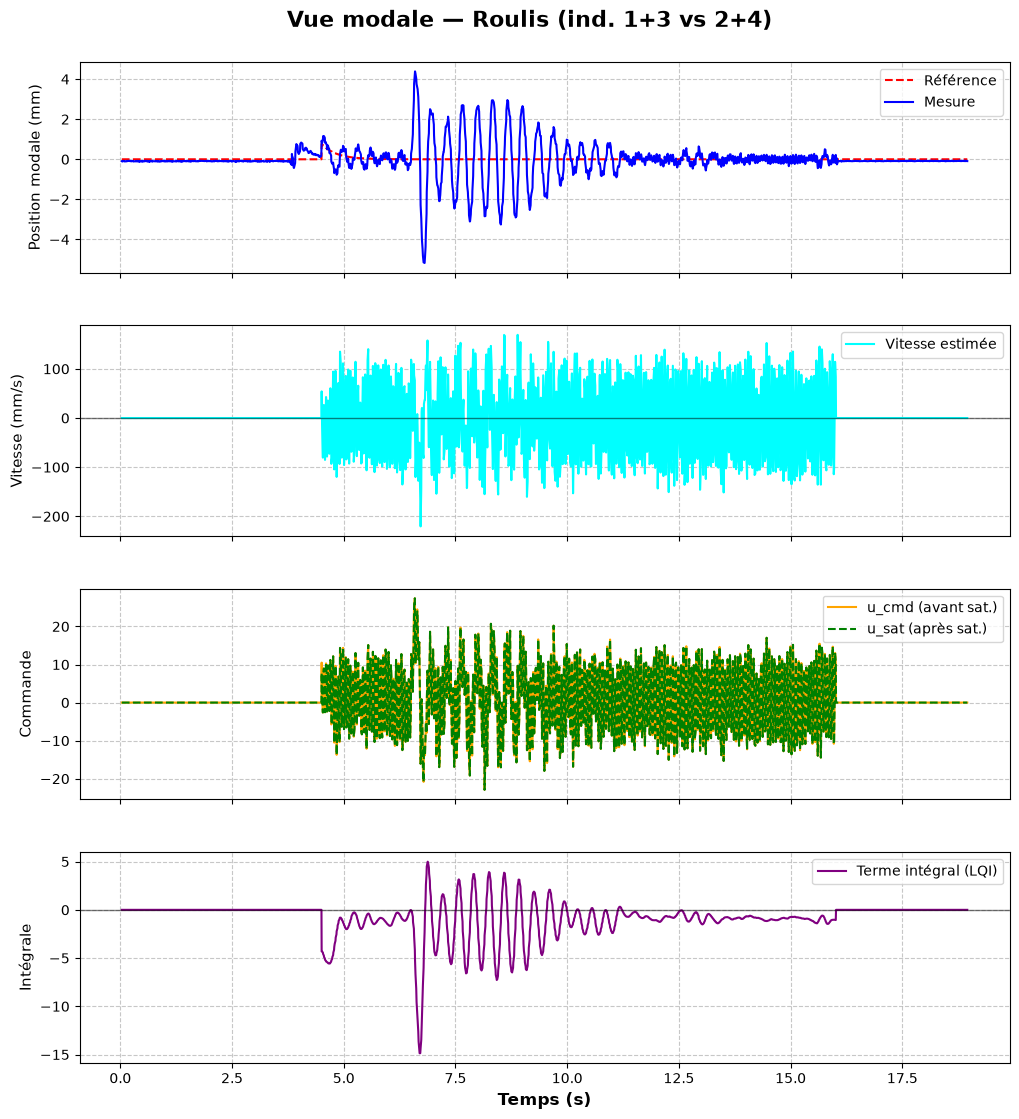
\includegraphics[width=1\linewidth]{assets/content/14-MesureMIMO/Oscillation/Roulis.png}
    \caption{Comportement du roulis avec une perturbation}
    \label{fig:RoulisOscillation}
\end{figure}

Le comportement par inducteur, avec une perturbation, est présenté de la \autoref{fig:Ind1Oscillation} à la \autoref{fig:Ind4Oscillation} :

\begin{figure}[H]
    \centering
    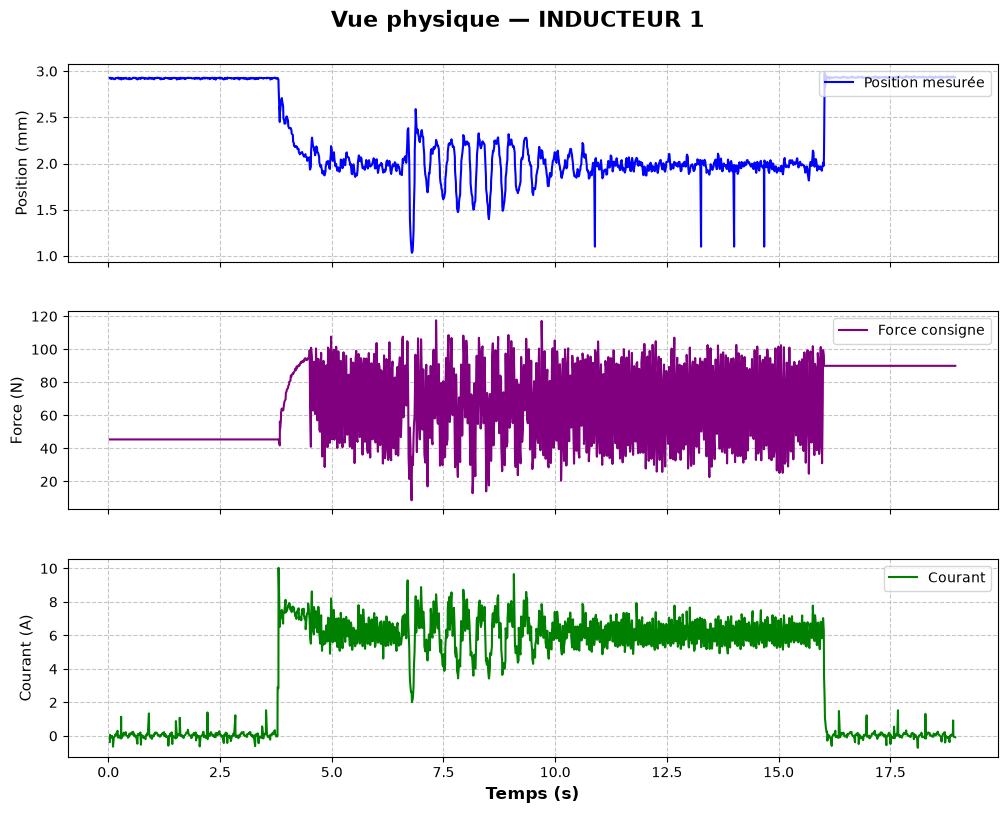
\includegraphics[width=1\linewidth]{assets/content/14-MesureMIMO/Oscillation/Ind1.png}
    \caption{Comportement de l'inducteur 1 avec une perturbation}
    \label{fig:Ind1Oscillation}
\end{figure}

\begin{figure}[H]
    \centering
    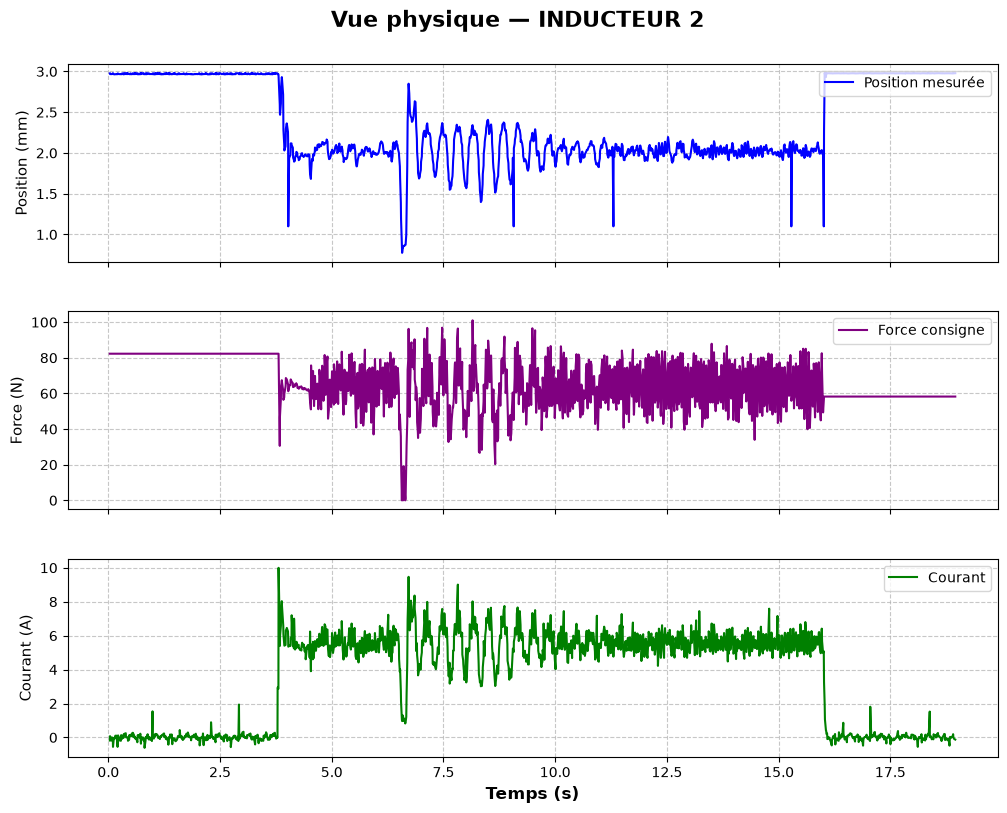
\includegraphics[width=1\linewidth]{assets/content/14-MesureMIMO/Oscillation/Ind2.png}
    \caption{Comportement de l'inducteur 2 avec une perturbation}
    \label{fig:Ind2Oscillation}
\end{figure}

\begin{figure}[H]
    \centering
    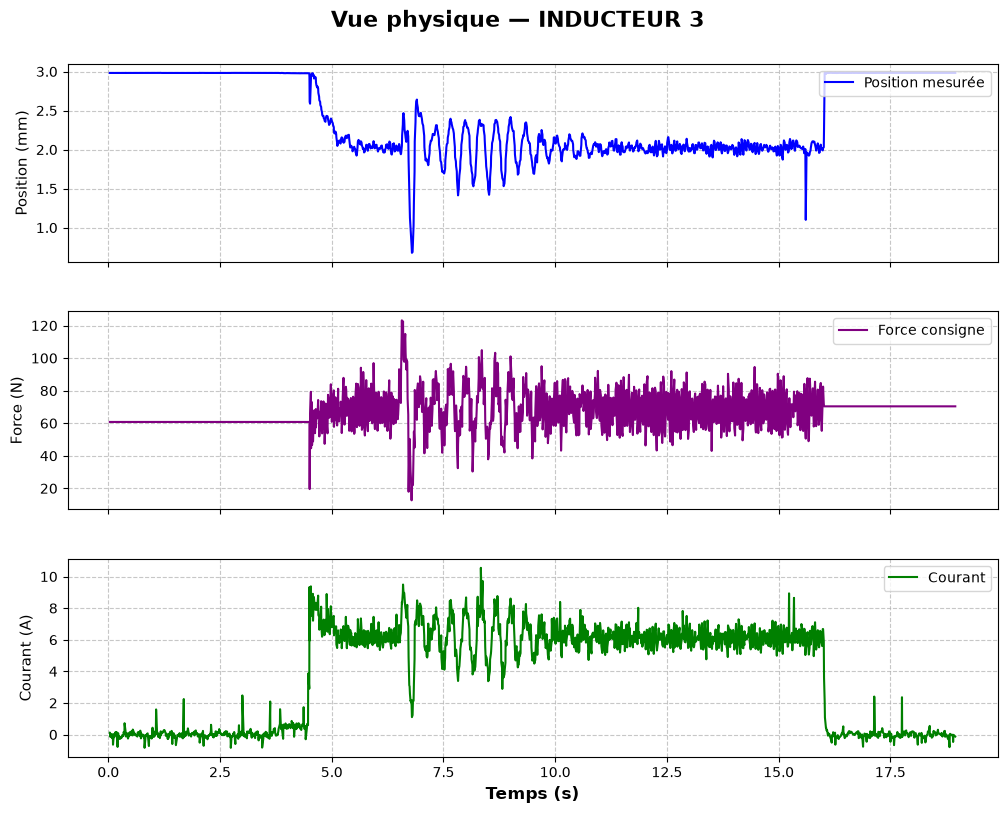
\includegraphics[width=1\linewidth]{assets/content/14-MesureMIMO/Oscillation/Ind3.png}
    \caption{Comportement de l'inducteur 3 avec une perturbation}
    \label{fig:Ind3Oscillation}
\end{figure}

\begin{figure}[H]
    \centering
    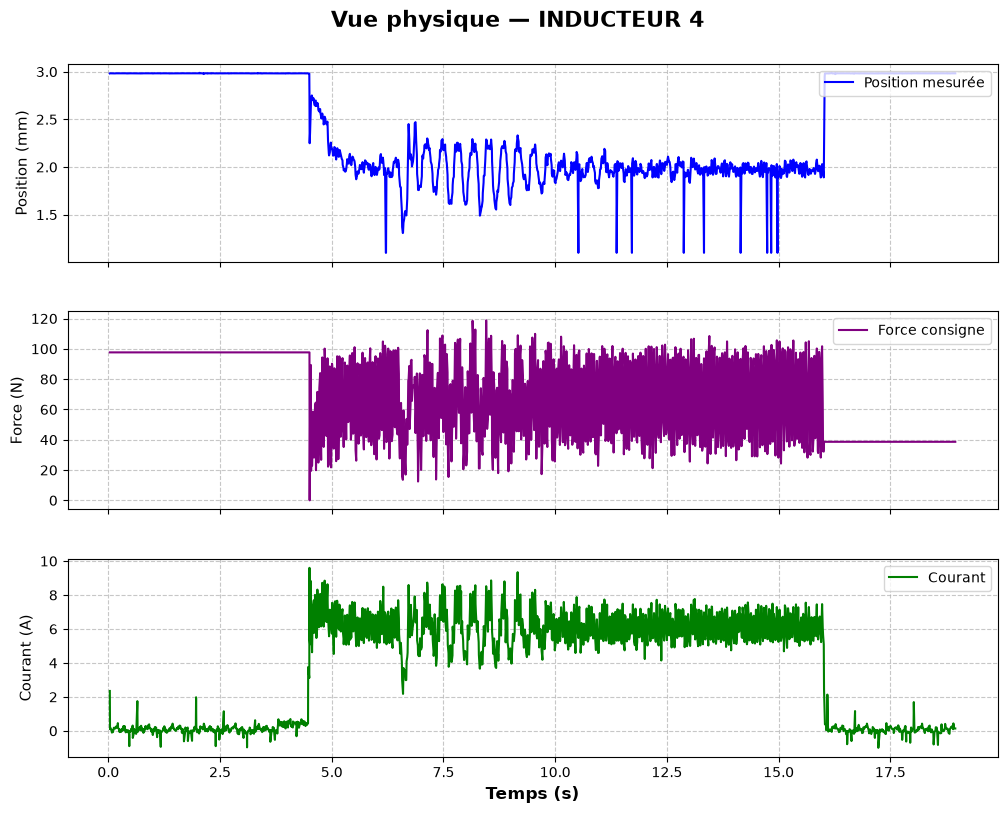
\includegraphics[width=1\linewidth]{assets/content/14-MesureMIMO/Oscillation/Ind4.png}
    \caption{Comportement de l'inducteur 4 avec une perturbation}
    \label{fig:Ind4Oscillation}
\end{figure}

Les forces émises avec une perturbation sont présentées dans la \autoref{fig:ForceOscillation} :

\begin{figure}[H]
    \centering
    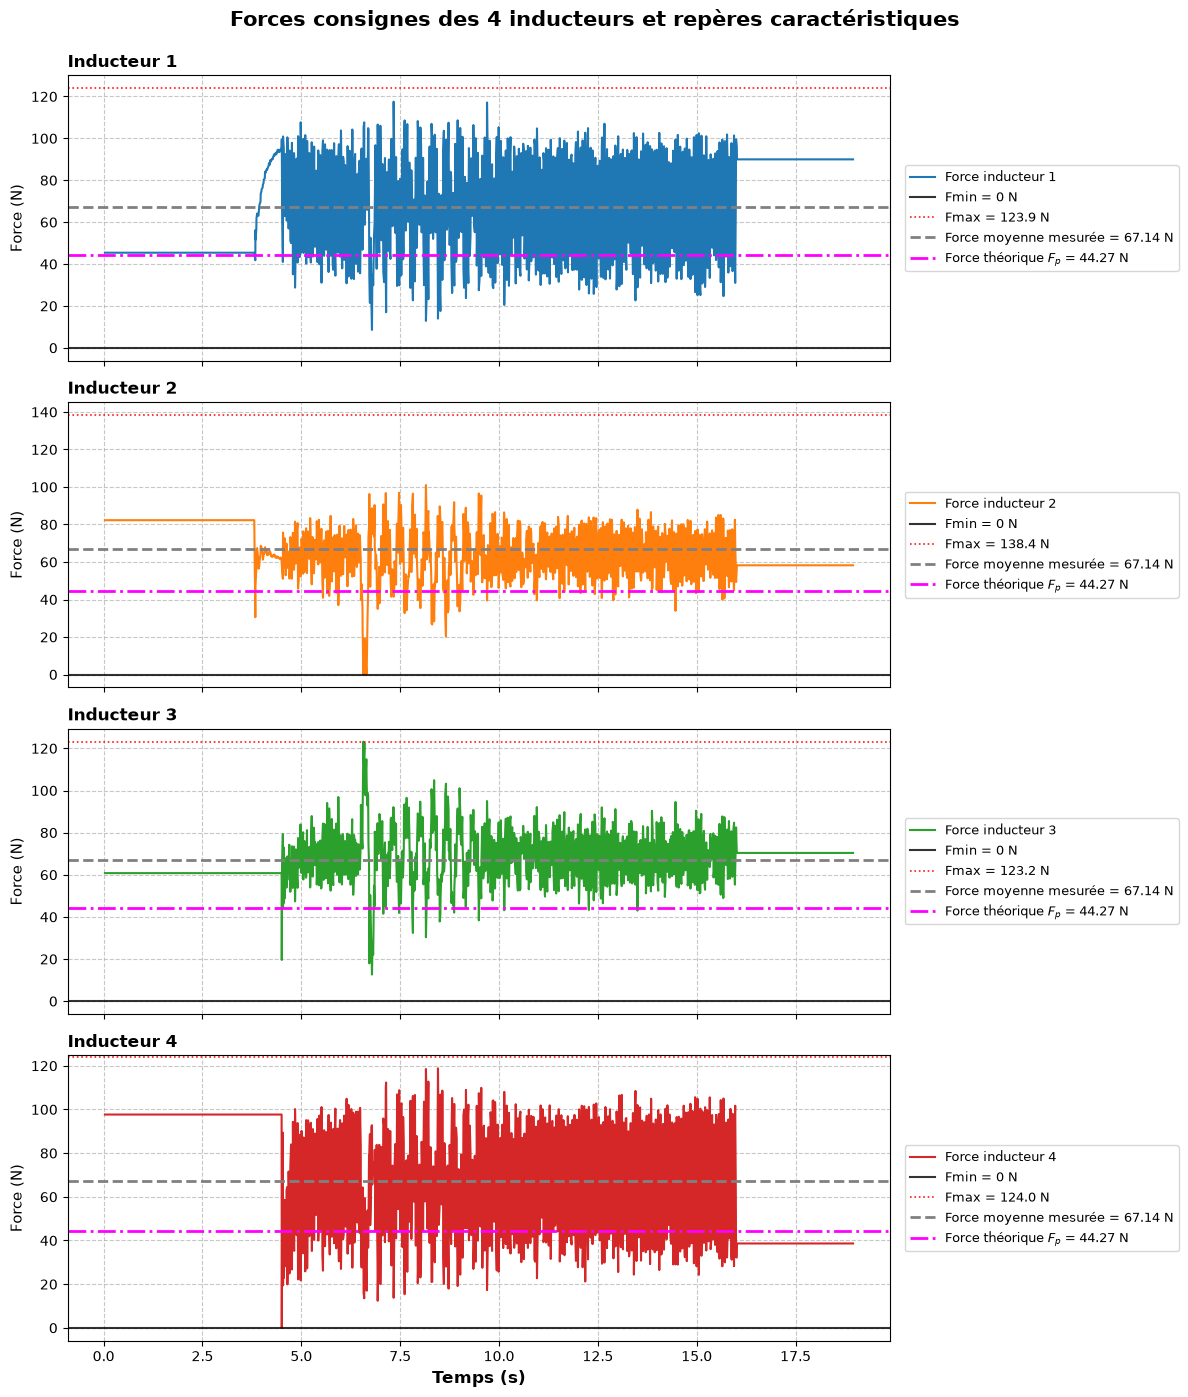
\includegraphics[width=1\linewidth]{assets/content/14-MesureMIMO/Oscillation/Force.png}
    \caption{Comportement des forces avec une perturbation}
    \label{fig:ForceOscillation}
\end{figure}

Comme précédemment, l'écart entre la force moyenne et la force théorique est calculé dans le \autoref{tab:forces_inducteurs_v4} :

\begin{table}[htbp]
    \centering
    \begin{tabular}{l cccc}
        \toprule
        \textbf{Inducteur} & \makecell[c]{\textbf{Force moyenne}                         \\ \textbf{[N]}} & \makecell[c]{\textbf{Force théorique $F_p$} \\ \textbf{[N]}} & \makecell[c]{\textbf{Écart} \\ \textbf{[N]}} & \makecell[c]{\textbf{Écart} \\ \textbf{[\%]}} \\
        \midrule
        1                  & 66.34                               & 44.27 & 22.07 & 49.85 \\
        2                  & 65.99                               & 44.27 & 21.71 & 49.04 \\
        3                  & 67.28                               & 44.27 & 23.01 & 51.97 \\
        4                  & 68.96                               & 44.27 & 24.69 & 55.76 \\
        \bottomrule
    \end{tabular}
    \caption{Comparaison des forces moyennes et théoriques par inducteur, avec une perturbation}
    \label{tab:forces_inducteurs_v4}
\end{table}

\subsection{Analyse des mesures}
Le système reste stable et en place.

La première mesure montre que le système parvient à se stabiliser autour de 2~mm d'entrefer. Il est intéressant de noter que le courant est plus important que prévu : le courant nominal avait été calculé à 4.48~A, alors qu'il se situe en réalité plus proche de 6~A. Cette augmentation est cohérente avec la force réellement demandée, qui se situe autour de 65~N, soit un écart d'environ 20 à 24~N par rapport à la force théorique. Bien que le système demande plus de force que prévu, il reste stable et l'alimentation parvient à fournir le courant nécessaire. Un élément encore inconnu forcerait donc le système à demander beaucoup plus de force que nécessaire. La masse comme les inductances ayant déjà été vérifiées, une cause tierce subsiste. Celle-ci n'a malheureusement pas été recherchée davantage, mais mériterait de l'être.

Les mesures modales montrent que le pompage et le tangage sont très stables : la plaque reste bien en l'air. Le roulis, en revanche, présente des oscillations. C'est dans ce degré de liberté que les oscillations sont les plus marquées.

La seconde mesure, avec perturbation, montre un système réactif : la perturbation est corrigée rapidement.

\section{Conclusion}
Ces mesures confirment le bon fonctionnement du système. Des oscillations subsistent, mais elles restent faibles. La régulation fonctionne donc correctement, même s'il resterait à améliorer le résultat.

Ces mesures montrent surtout l'intérêt de poursuivre les recherches sur la régulation MIMO, qui donne de bien meilleurs résultats que le SISO.
